% little trick to replace lib.tex by this
\renewcommand{\doctitle}[1]{
	\chapter{#1}
}
\renewcommand{\biblio}[1]{}
\doctitle{Fonctionnement général d'un synthétiseur}

Le synthétiseur analogique que nous devons concevoir
est divisé en 3 blocs principaux (voir figure \ref{fig:gf-global}).

\begin{figure}[ht]
	\centering
	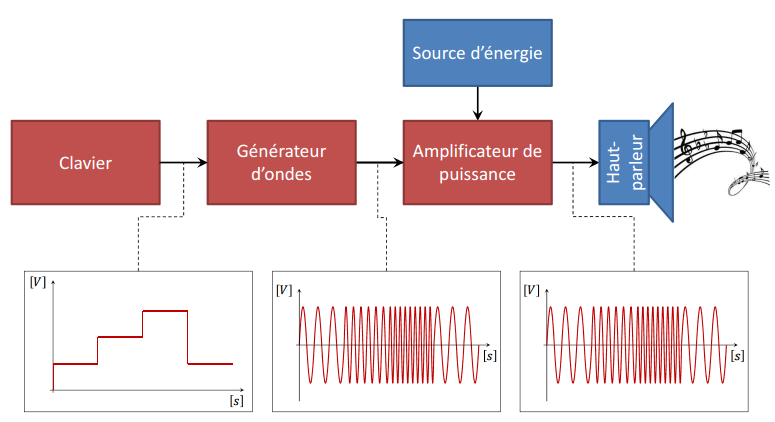
\includegraphics[scale=0.6]{img-gf/gf-global.png}
	\caption{Schéma blocs global du synthétiseur (source : Bruno Dehez.}
	\label{fig:gf-global}
\end{figure}

Premièrement, il y a bien sur un clavier. Ce clavier est simplement
composé de diviseurs résistifs et de boutons poussoirs. Il doit
permettre de générer différentes tensions continues, chacune
correspondant à une note.

Cette tension continue sera ensuite appliquée en entrée du générateur
d'onde. Ce générateur se décompose en deux blocs (voir figure
\ref{fig:gf-generator}). Un oscillateur contrôlé en tension 
(\textit{voltage controlled oscillator}, ou VCO en anglais) va dans
un premier temps transformer cette tension d'entrée continue
en un signal périodique (dans notre cas un signal triangulaire) 
dont la fréquence sera directement proportionnelle
à la tension d'entrée, de telle sorte que
\unit{1}{\milli\volt} corresponde à \unit{1}{\hertz}. Ensuite, un filtre
transformera ce signal triangulaire en signal sinusoïdal
\footnote{On comprend ici l'intérêt de générer un signal triangulaire plutôt
qu'un signal en dents de scie ou un signal carré. En effet, filtrer
de tels signaux pour obtenir un signal sinusoïdal engendrera
une plus grande perte de puissance qu'à partir d'un signal
triangulaire.}.

\begin{figure}[ht]
	\centering
	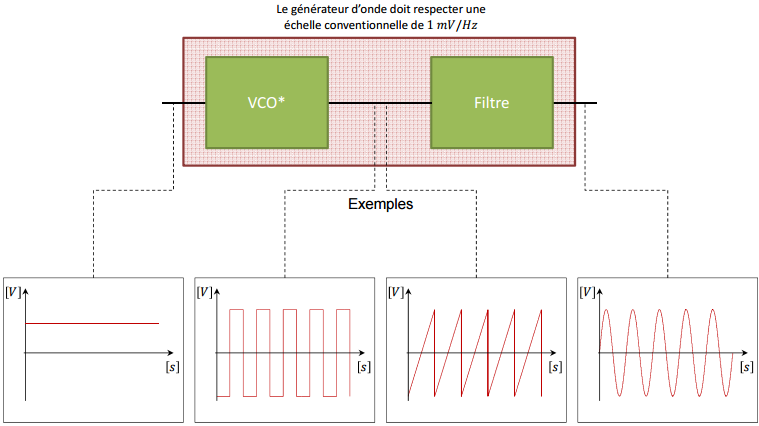
\includegraphics[scale=0.6]{img-gf/gf-generator.png}
	\caption{Schéma-bloc du générateur d'onde (source : Bruno Dehez).}
	\label{fig:gf-generator}
\end{figure}

Afin d'obtenir un son à partir de ce signal sinusoïdal, il
va falloir l'appliquer en entrée d'un haut-parleur. Mais avant
cela, il va falloir l'amplifier. Pour ce faire, nous allons
utiliser un amplificateur de classe D (voir figure
\ref{fig:gf-ampli}). Un tel amplificateur
a un très bon rendement, il consomme peu de puissance. Cependant,
pour que cet amplificateur fonctionne correctement, il faut
lui appliquer un signal carré avec une tension basse nulle en entrée. Pour transformer
notre signal sinusoïdal en signal carré, nous allons utiliser un
système de modulation de largeur d'impulsion (ou MLI). Le MLI
transforme son entrée sinusoïdale en un signal carré dont la
valeur moyenne est égale à l'entrée. Ce
signal carré est ensuite amplifié par l'étage de puissance
et filtré afin d'obtenir à nouveau un signal sinusoïdal que
l'on pourra cette fois directement appliqué en entrée du haut-parleur.

% N'apportait rien selon Claude Oestges
%\begin{figure}[ht]
	%\centering
	%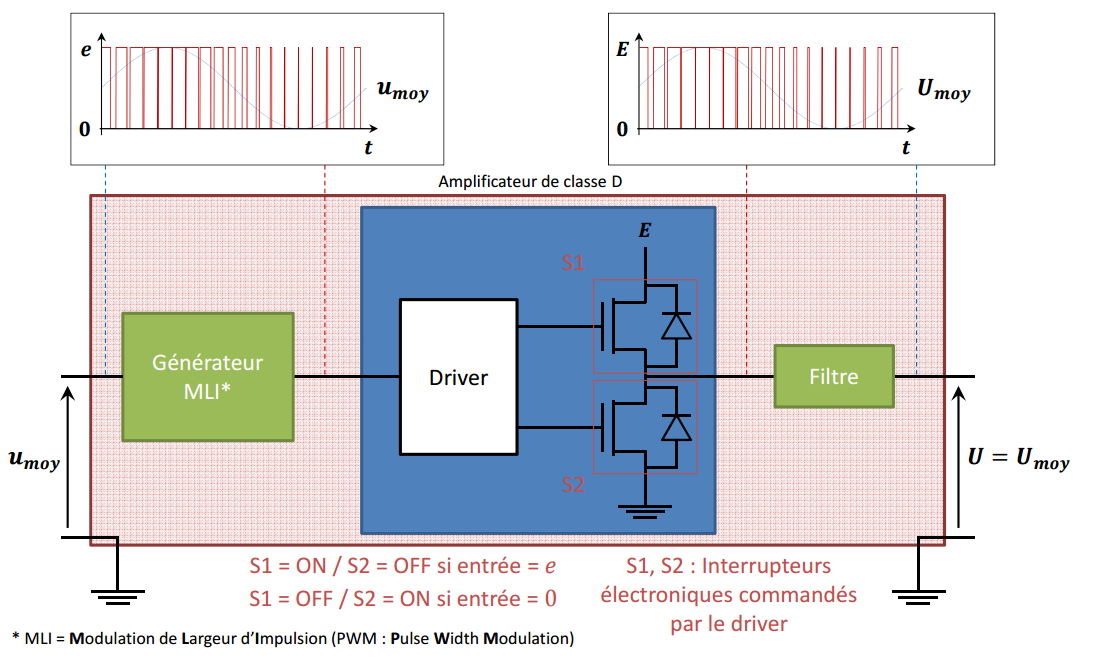
\includegraphics[scale=0.55]{img-gf/gf-ampli.png}
	%\caption{Schéma blocs de l'amplificateur (source : Bruno Dehez).}
	%\label{fig:gf-ampli}
%\end{figure}

\end{document}
